\section{k-Server-Problem}

\begin{takeaway}
    \item k-Server-Problem
    \item Potentialfunktionen, amortisierte Kosten
    \item Greedy, Double Coverage
\end{takeaway}

\paragraph{Motivation}
Bewege Objekte in einem Raum zu bestimmten Punkten.
Z.B. Polizisten von Dienststellen zu crime scenes, oder Taxis zu Kunden.

``Heiliger Gral'' der Online-Algorithmen, wie TSP für Approximations-Algorithmen oder SAT für NP.

\paragraph{Metrischer Raum}
Sei $S$ eine Menge von Punkten, sei $\dist : S \times S \mapsto \mathbb{R}$ eine Distanzfunktion.
$\mathcal{M}(S, \dist)$ ist ein \emph{metrischer Raum} falls gilt:
Definitheit, Symmetrie, Dreiecksungleichung.

Beispiel: Euklidischer Raum. Vollständige, gewichtete, ungerichtete Graphen mit Dreiecksungleichung.
\\
Beobachtung: Alle Graphen mit Kastenkosten $\in \{1, 2\}$ erfüllen die Dreiecksungleichung.

\paragraph{k-Server}
Sei $\mathcal{M}(S, \dist)$ ein metrischer Raum.
Sei $s_1, ..., s_k$ Server als Punkte in $S$.
Sei eine Multimenge $C_i \subseteq S$ mit $|C_i|=k$ eine \emph{Konfiguration} von Servern in Zeitschritt $i$.
\\
Die \emph{Distanz} \footnote{Achtung Verwechslungsgefahr!}
zwischen $C_r$ und $C_t$ sind die Kosten eines minimalen Matchings zwischen ihnen.

Eine Instanz $I = (x_1, ..., x_n)$ fragt Punkte an, so dass in Zeitschritt $i$ ein Server nach $x_i$
bewegt werden muss (falls dort noch keiner steht).

Ziel: $\min \sum_i costMinMatching(C_i, C_{i+1})$

\paragraph{Träge}
Ein Online-Algorithmus für k-Server heisst \emph{träge (lazy)} wenn er nur dann einen Server bewegt,
wenn auf $x_i$ noch kein Server steht.
Auch bewegt er pro Zeitschritt maximal einen Server.

Dies erleichtert die Analyse. Gleichzeitig gilt (Satz): \\
Jeder c-kompetitive OA für k-Server kann in einen trägen OA umgewandelt werden der auch c-kompetitiv ist.

\paragraph{k-Server als Verallgemeinerung von Paging}
Cache $k$, Hauptspeicher $m$ $\longrightarrow$ vollständiger Graph mit $m$ Knoten und initial
Servern auf $(v_1, ..., v_k)$. Angefragte Punkte = angefragte Seiten.

Daraus folgt eine untere Schranke (Satz):
Es existiert ein metrischer Raum so dass kein deterministischer OA für k-Server besser als k-kompetitiv ist.
\\
Frage: für Paging ist die Schranke scharf, d.h. wir kennen einen Algo (z.B. FIFO).
Können wir für k-Server auch einen Algo konstruieren?

\paragraph{k-Server Vermutung(en)}
\begin{itemize}
    \item Es existiert ein k-kompetitiver deterministischer OA für k-Server.
    \item Es existiert ein im Erwartungswert $\Theta(\log k)$-kompetitiver randomisierter OA für k-Server.
\end{itemize}
D.h. die untere Schranke ist erreichbar.
Wenn dies wahr ist, dann ist k-Server genauso schwer wie Paging!
Aktueller Stand: $2k-1$.

\paragraph{Greedy-Algorithmus}
Bewege immer den Server der am nähesten dran ist.

\underline{Satz:}
$Greedy$ ist nicht kompetitiv für k-Server.

\underline{Beweis:}
Siehe Instanz in \autoref{k-server-greedy}.
Hier gilt $\frac{cost(Greedy(I))}{cost(I)} = \frac{n}{2}$, d.h. es gibt keine Konstante $c$
so dass $Greedy$ $c$-kompetitiv wäre.

\begin{figure}[h]
    \centering
    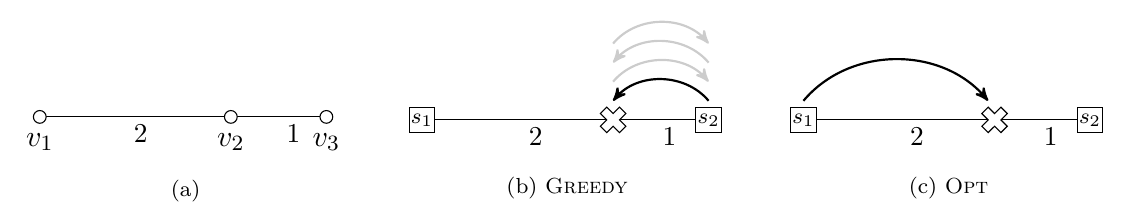
\includegraphics[width=0.8\textwidth]{images/k-server-greedy.png}
    \caption{k-Server: $Greedy$ versus $Opt$}
    \label{k-server-greedy}
\end{figure}


\subsection{Potentialfunktionen}

\paragraph{Motivation}
Kompetivität $c$ abschätzen über die \emph{amortisierten Kosten}.
Statt dass $cost(A(I)) \leq c \cdot cost(Opt(I)) + \alpha$ für alle $I$ gelten muss,
wollen wir zeigen dass $cost(A(x_i)) \leq c \cdot cost(Opt(x_i)) + \alpha$ für alle $x_i$ gilt.
\\
Dann können wir erlauben dass $A$ in einigen Zeitschritten mehr als $c$-mal schlechter ist als $Opt$,
solange er in anderen wieder weniger schlecht ist.

\paragraph{Potentialfunktion}
Sei $\mathcal{K}_{Alg}$ die Menge aller \emph{Konfigurationen} von $A$ auf Instanz $I$
und sei $\mathcal{K}_{Opt}$ die Menge aller Konfigurationen eines beliebigen, aber festen, $Opt$.
\footnote{Konfiguration: nach aussen sichtbar, nicht der interne state der Turingmaschine.
Z.B. Position der Server, Seiten im Cache.}

Dann ist eine \emph{Potentialfunktion} $\Phi$:
$$
\Phi \cl  \mathcal{K}_{Alg} \times \mathcal{K}_{Opt} \mapsto \R
\qquad \text{oder} \qquad
\Phi \cl \I \mapsto \R
$$
Die Konfigurationen sind eindeutig durch die Eingabe gegeben, daher die beiden Darstellungen.

Das \emph{Potential} in Zeitschritt $i$ ist $\Phi(x_i)$.

Die \emph{amortisierten Kosten} (vgl. \emph{tatsächliche Kosten}) sind:
$$ amcost(A(x_i)) := cost(A(x_i)) + \Phi(x_i) - \Phi(x_{i-1})$$

\paragraph{Satz}
Falls
$$ \exists \beta \in \R^+ \text{konstant} \; \forall i \in [1,n] \cl 0 \leq \Phi(x_i) \leq \beta
\quad \wedge \quad
amcost(A(x_i)) \leq c \cdot cost(Opt(x_i))
$$
dann ist $A$ $c$-kompetitiv für $\Pi$.

Dies lässt sich verallgemeinern dass $\Phi$ negativ werden darf, solange es trotzdem durch
eine Konstante beschränkt ist.

\underline{Beweis:}
Siehe Skript S.48. Kurz:
$$ cost(A(I)) = \sum_{i=1}^n cost(A(x_i)) = \dots \leq c \cdot cost(Opt(I)) + \beta $$
Amortisierte Kosten einsetzen, dann Potentiale auscanceln. Dann $\alpha := \beta$ setzen.

\subsection{k-Server auf der Linie}

\paragraph{Die Line}
Betrachte den metrischen Raum $\M_{[0,1]} = ([0,1], \dist)$ mit $\dist(x,y) = |x-y|$,
d.h. den Zahlenstrahl der reellen Zahlen zwischen 0 und 1.

\paragraph{Double Coverage-Algorithmus}
Idee: bewege von beiden Seiten eine Server je um die selbe Distanz in Richtung $x_i$.
Nicht träge!

\begin{figure}[h]
    \centering
    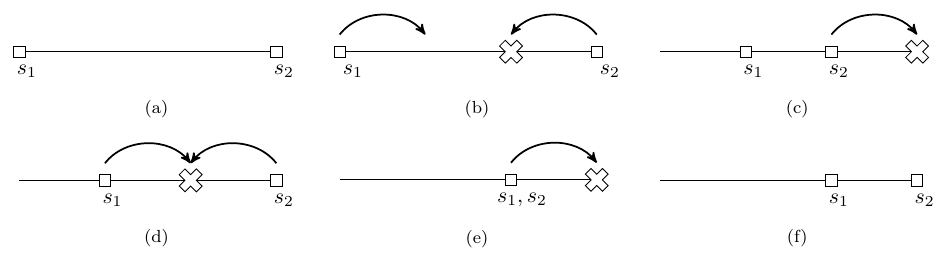
\includegraphics[width=0.8\textwidth]{images/k-server-double-coverage.png}
    \caption{k-Server: $DoubleCoverage$ anhand von $Greedys$ worst-case Beispiel}
    \label{k-server-double-coverage}
\end{figure}

\begin{algorithm}[h]
\caption{Double Coverage (ein Zeitschritt)}
\begin{algorithmic}
    \State $s \gets x_i$
    \State $s_{rechts} \gets \lambda; s_{links} \gets \lambda$
    \State $s_{rechts} \gets $ Server direkt rechts neben $s$
    \State $s_{links} \gets $ Server direkt links neben $s$
    \If{$s_{rechts} = \lambda$}
        \State output "Bewege $s_{links}$ zu $s$"
    \ElsIf{$s_{links} \gets \lambda$}
    \State output "Bewege $s_{rechts}$ zu $s$"
    \Else
    \State $d \gets \min \{ \dist(s_{rechts} , s), \dist(s_{links} , s) \}$
    \State output "Bewege $s_{rechts}$ um $d$ nach links und $s_{links}$ um d nach rechts"
    \EndIf
\end{algorithmic}
\end{algorithm}

\paragraph{Satz}
$DoubleCoverage$ ist k-kompetitiv für k-Server auf $\M_{[0,1]}$.

\underline{Beweis}:
Siehe Skript S.49ff.

Ziel: Definiere Potentialfunktion $\Phi$ so dass die Bedingungen vom Satz gelten.
\\
Sei $K_{DC} = \{p_1^{DC}, \dots , p_k^{DC}\}$ eine Konfigurationen von DC (d.h. die Positionen seiner Server).
Sei $K_{Opt}$ analog.
Seien $M_{\min} (K_{DC}, K_{Opt})$ die Kosten eines minimalen Matchings
und sei $DC(K_{DC})$ die Summe der paarweisen Distanzen aller Server von DC.
Wir definieren:
$$\Phi (K_{DC}, K_{Opt}) := k \cdot M_{\min} (K_{DC}, K_{Opt}) + DC(K_{DC}) $$

Beobachte: $\Phi$ ist positiv, konstant, und hängt nicht von $n$ ab. Konkret (Bedingung 1):
\footnote{Recall that wir uns in $\M_{[0,1]}$ bewegen, d.h. alle Distanzen zwischen zwei Punkten sind $\leq 1$.}
$$ 0 \leq \Phi (K_{DC}, K_{Opt}) \leq k \cdot k + \binom{k}{2} \leq 2 k^2 := \beta $$

Zeige nun dass $\forall i$ gilt $(\star)$:
$ \Phi(x_i) - \Phi(x_{i-1}) \leq k \cdot cost(Opt(x_i)) - cost (DC(x_i)) $ (Bedingung 2).
\\
Schätze dazu ab wie sich das Potential verändert (durch die Änderung der Konfiguration)
wenn erst $Opt$ und dann $DC$ einen Zug machen.

Der Zug von $Opt$ vergrössert $\Phi$ um $\leq k \cdot cost(Opt(x_i))$
(maximal ein Server wird um $cost(Opt(x_i))$ bewegt, nur $k \cdot M_{\min}$ ist affected).

Der Zug von $DC$ verändert $\Phi$ um:
\begin{itemize}
    \item[Fall 1:] $x_i$ ist ``ganz aussen''. OBdA wird $s_{rechts}$ nach links verschoben.
        Der zweite Summand vergrössert das Potential um $\leq (k-1) \cdot cost(DC(x_i))$.
        \\
        OBdA existiert ein minimales Matching das $s$ (von $Opt$ bereits nach $x_i$ bewegt)
        und $s_{rechts}$ matched -- siehe Fallunterscheidung).
        D.h. die Kosten von $k \cdot M_{\min}$ verringern sich um $k \cdot cost(DC(x_i))$.
        \\
        $\implies$ insgesamt gilt $(\star)$
    \item[Fall 2:] $x_i$ ist zwischen $s_{links}$ und $s_{rechts}$.
        Der zweite Summand wird um $cost(DC(x_i))$ kleiner (da sich $s_{links}, s_{rechts}$ näher kommen).
        OBdA sind vor dem Zug von $DC$ $s$ und $s_{links}$ (oder $s$ und $s_{rechts}$) gematched.
        Dies verringert die Kosten von $M_{\min}$ um $cost(DC(x_i))/2$.
        \\
        Der andere wird mit einem $s'''$ von $Opt$ gematched.
        Hier erhöhen sich die Kosten um $\leq cost(DC(x_i))/2$.
        D.h. der erste Summand bleibt gleich oder wird kleiner.
        \\
        $\implies$ insgesamt gilt $(\star)$
\end{itemize}
$\implies$ Bedingung 1 + 2 vom Satz erfüllt $\implies$ $DC$ ist k-kompetitiv.
